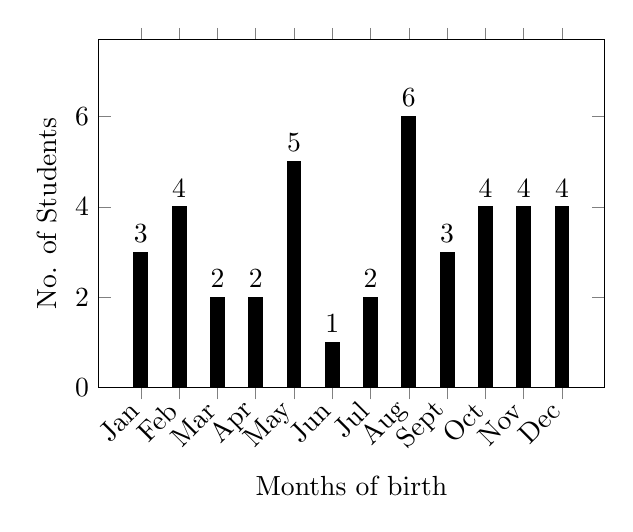
\begin{tikzpicture}
\begin{axis}[
ybar,
ymin=0,
width=8cm,
height=6cm,
ymax=7,
bar width=5pt,
ylabel={No. of Students},
xlabel={Months of birth},
nodes near coords,
symbolic x coords={Jan,Feb,Mar,Apr,May,Jun,Jul,Aug,Sept,Oct,Nov,Dec},
xtick = data,
x tick label style={rotate=45,anchor=east},
enlarge y limits={value=0.1,upper},
legend pos=north east,
]
\addplot[fill=black] coordinates {(Jan,3) (Feb,4)(Mar,2) (Apr,2)(May,5)(Jun,1)(Jul,2)(Aug,6)(Sept,3)(Oct,4)(Nov,4)(Dec,4)};
\end{axis}
\end{tikzpicture}
